\documentclass{article}
\usepackage{tikz}
\usetikzlibrary{angles}

\begin{document}

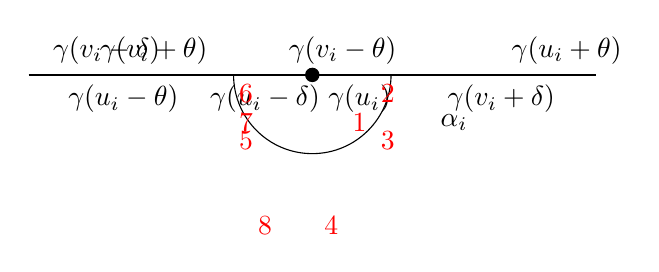
\begin{tikzpicture}[scale=1.2]
    % Define coordinates for the points
    \coordinate (A) at (-3, 0);
    \coordinate (B) at (-1, 0);
    \coordinate (C) at (0, 0);
    \coordinate (D) at (1, 0);
    \coordinate (E) at (3, 0);

    % Draw the segments
    \draw[black, thick] (A) -- node[below] {$\gamma(u_i - \theta)$} (B);
    \draw[black, thick] (B) -- node[below] {$\gamma(u_i - \delta)$} (C);
    \draw[black, thick] (C) -- node[below] {$\gamma(u_i)$} (D);
    \draw[black, thick] (D) -- node[below] {$\gamma(v_i + \delta)$} (E);
    \draw[black, thick] (D) -- node[above right] {$\gamma(u_i + \theta)$} (E);
    \draw[black, thick] (B) -- node[above left] {$\gamma(v_i - \theta)$} (E);
    \draw[black, thick] (A) -- node[above left] {$\gamma(v_i - \delta)$} (C);
    \draw[black, thick] (A) -- node[above left] {$\gamma(v_i + \theta)$} (D);

    % Mark the intersection point
    \filldraw[black] (C) circle (2pt);

    % Draw angles with labels
    \pic[draw, angle radius=1cm, angle eccentricity=1.2] {angle = A--C--E};
    \node at (1.5, -0.5) {$\alpha_i$};

    % Number the points in red
    \node[red] at (0.5, -0.5) {$1$};
    \node[red] at (0.8, -0.2) {$2$};
    \node[red] at (0.8, -0.7) {$3$};
    \node[red] at (0.2, -1.6) {$4$};
    \node[red] at (-0.7, -0.7) {$5$};
    \node[red] at (-0.7, -0.2) {$6$};
    \node[red] at (-0.7, -0.5) {$7$};
    \node[red] at (-0.5, -1.6) {$8$};
\end{tikzpicture}

\end{document}